\chapter{Regulator obiektu}
Drugim zadaniem wchodzącym w skład projektu była implementacja działającego regulatora PID. Miał być to regulator równoległy bez odsprzęgania, innymi słowy składał się on z dwóch regulatorów PID nie ingerujących we własne działanie. Każdy z nich otrzymywał na wejście uchyb jednego z wyjść i generował odpowiednie sterowanie. Wyjścia i wejścia zostały przez nas sparowane w następujący sposób: $C_A$ z $F_C$ oraz $T$ z $C_{Ain}$.
Decyzja ta została podyktowana charakterystyką działania obiektu określoną w pierwszej części projektu, według której zwiększenie sterowania $C_{Ain}$ powodowało spadek wartości wyjścia $C_A$, a zwiększenie $T$. Reakcja dla drugiego wyjścia była odwrotna.

Mając określone wejścia i wyjścia regulatorów mogliśmy przystąpić do implementacji w programie OVATION. Zgodnie z instrukcją prowadzącego posłużyliśmy się w tym celu blokiem regulatora PID obecnym systemie. Dodatkowo skorzystaliśmy z przełącznika binarnego używanego w arkuszu modelu obiektu służącego do przełączania trybów sterowania: manualnego i regulowanego. W trybie manualnym regulatory zostają odcięte, a podawany na nie uchyb jest zerowany.

\begin{figure}[h!]
	\centering
	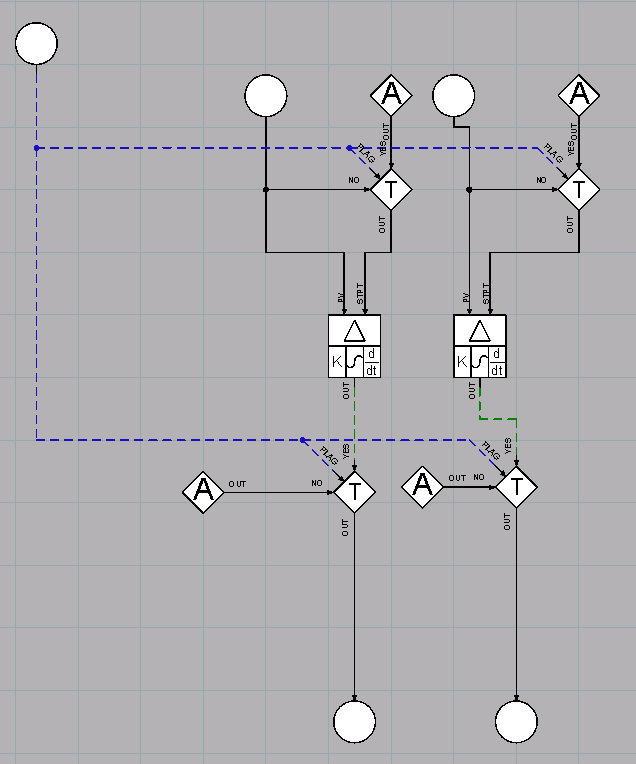
\includegraphics[width=.6\linewidth]{img/PID.png}
	\label{ch2:regulator}
	\caption{Model regulatora wykonany w programie OVATION}
\end{figure}
\newpage
Blok PID zawierał cztery parametry, które należało odpowiednio dobrać w celu osiągnięcia optymalnej regulacji. Ze względu na fakt, że strojenie regulatorów bezpośrednio na zaimplementowanym obiekcie mogłoby zając więcej czasu niż mieliśmy, zdecydowaliśmy się dobrać nastawy z użyciem modelu wykonanego w programie Matlab i klasy regulatora, udostępnionej przez prowadzącego, bliźniaczo podobnej w działaniu do bloku obecnego w OVATION. Po uzyskaniu zadowalających wyników, nastawy regulatorów przeniesione zostały do symulatora OVATION. Ze względu na fakt, że Matlab oraz OVATION używają innych rozmiarów zmiennych liczbowych, działanie symulacji nie było całkowicie identyczne z danymi uzyskanymi w programie Matlab. Z tego powodu nastawy regulatorów zostały przez nas udoskonalone na podstawie wyników działania symulacji. Poniżej zamieszczamy tabelę z ostatecznymi parametrami obydwu regulatorów.

\begin{table}[h!]
	\centering
	\begin{tabular}{|c|c|c|c|c|c|}
		\hline
		Zmienna regulowana&Wyjście&K&Ti&Kd&Td\\\hline
		$C_A$&$F_C$&10&0,55&80&10\\\hline
		$T$&$C_{Ain}$&0,002&600&0,2&1,8\\\hline
	\end{tabular}
\label{tab:pid}
\caption{Nastawy regulatorów PID}
\end{table}

Na koniec pozostało jeszcze zadanie udokumentowania działania zaimplementowanego przez nas układu regulacji. Poniżej przedstawiamy wyniki działania regulatorów w formie wykresów.

\begin{figure}[h!]
	\centering
	\includegraphics[width=.8\linewidth]{img/pid.eps}
	\label{ch2:pid}
	\caption{Działanie regulatora PID regulującego wyjście $C_A$}
\end{figure}
